% https://www.sharelatex.com/blog/2013/08/27/tikz-series-pt1.html

\documentclass{standalone}

\usepackage{tikz}
\usetikzlibrary{shapes.geometric, arrows,positioning,calc}

\tikzstyle{startstop} = [rectangle, rounded corners, minimum width=2cm, minimum
height=0.5cm, align=center, draw]

\tikzstyle{io} = [trapezium, trapezium left angle=70, trapezium right angle=110, align=center, draw]

\tikzstyle{process} = [rectangle, align=center, draw]

\tikzstyle{oval}=[ellipse, align=center, draw]

\tikzstyle{decision} = [shape aspect=2,diamond, align=center, draw]

\tikzstyle{arrow} = [thick,->,>=stealth]
\tikzstyle{dotArrow} = [dotted, ->, >=stealth]
\tikzstyle{line} = [-]




\begin{document}
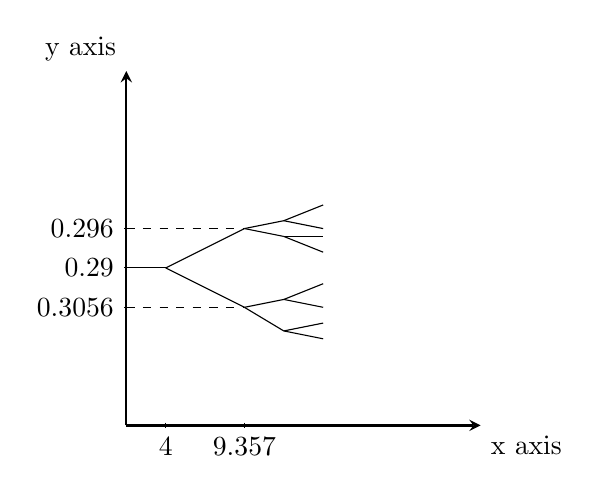
\begin{tikzpicture}
  \draw[thick,->, >=stealth] (0,0) -- (4.5,0) node[anchor=north west] {x axis};
  \draw[thick,->, >=stealth] (0,0) -- (0,4.5) node[anchor=south east] {y axis};
  
  %\foreach \x in {0,1,2,3,4}
  %\draw (\x cm,1pt) -- (\x cm,-1pt) node[anchor=north] {$\x$};
  
  %\foreach \y in {0,1,2,3,4}
  %\draw (1pt,\y cm) -- (-1pt,\y cm) node[anchor=east] {$\y$};

  \foreach \y in {1.5}
  \draw (1pt,\y cm) -- (-1pt,\y cm) node[anchor=east] {0.3056};
  
  \foreach \y in {2}
  \draw (1pt,\y cm) -- (-1pt,\y cm) node[anchor=east] {0.29};

  \foreach \y in {2.5}
  \draw (1pt,\y cm) -- (-1pt,\y cm) node[anchor=east] {0.296};

  \foreach \x in {0.5}
  \draw (\x cm,1pt) -- (\x cm,-1pt) node[anchor=north] {4};

  \foreach \x in {1.5}
  \draw (\x cm,1pt) -- (\x cm,-1pt) node[anchor=north] {9.357};

  \draw (0, 2) -- (0.5, 2);
  
  \draw (0.5, 2) -- (1.5, 1.5);
  \draw (0.5, 2) -- (1.5, 2.5);

  \draw (1.5, 2.5) -- (2, 2.6);
  \draw (1.5, 2.5) -- (2, 2.4);

  \draw (1.5, 1.5) -- (2, 1.6);
  \draw (1.5, 1.5) -- (2, 1.2);

  \draw (2, 2.6) -- (2.5, 2.8);
  \draw (2, 2.6) -- (2.5, 2.5);

  \draw (2, 2.4) -- (2.5, 2.4);
  \draw (2, 2.4) -- (2.5, 2.2);

  \draw (2, 1.6) -- (2.5, 1.8);
  \draw (2, 1.6) -- (2.5, 1.5);

  \draw (2, 1.2) -- (2.5, 1.3);
  \draw (2, 1.2) -- (2.5, 1.1);

  %\draw[dotted] (2.5, 0) -- (2.5, 3.5);
  %\draw[dotted] (2.6, 0) -- (2.6, 3.5);
  %\draw[dotted] (2.7, 0) -- (2.7, 3.5);
  %\draw[dotted] (2.8, 0) -- (2.8, 3.5);
  %\draw[dotted] (2.9, 0) -- (2.9, 3.5);
  %\draw[dotted] (3.0, 0) -- (3.0, 3.5);
  %\draw[dotted] (3.1, 0) -- (3.1, 3.5);
  %\draw[dotted] (3.2, 0) -- (3.2, 3.5);
  %\draw[dotted] (3.3, 0) -- (3.3, 3.5);
  %\draw[dotted] (3.4, 0) -- (3.4, 3.5);  
  
  

  \draw[dashed] (0, 2.5) -- (1.5, 2.5);
  \draw[dashed] (0, 1.5) -- (1.5, 1.5);
  
  
  
\end{tikzpicture}
\end{document}



%%% Local Variables:
%%% mode: latex
%%% TeX-master: t
%%% End:
